\documentclass[convert={density=300,size=1080x800,outext=.png}]{standalone}

\usepackage{amsfonts}

\usepackage{tikz}
\usetikzlibrary{backgrounds}

\definecolor{paleaqua}{HTML}{B4D4EE}

\newcommand{\cR}{\mathcal{R}}

\begin{document}
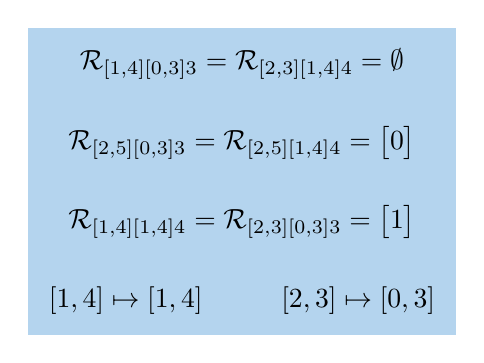
\begin{tikzpicture}[background rectangle/.style={fill=paleaqua}, show background rectangle]
  \node at (0,3) {$\cR_{[1,4][0,3]3} = \cR_{[2,3][1,4]4} = \emptyset$};
  \node at (0,2) {$\cR_{[2,5][0,3]3} = \cR_{[2,5][1,4]4} = \big[0 \big]$};
  \node at (0,1) {$\cR_{[1,4][1,4]4} = \cR_{[2,3][0,3]3} = \big[1 \big]$};
  \node at (0,0) {$[1,4] \mapsto [1,4] \hspace{1cm}
[2,3]\mapsto [0,3]$};
\end{tikzpicture}
\end{document}
